% FID values for run10 and run11
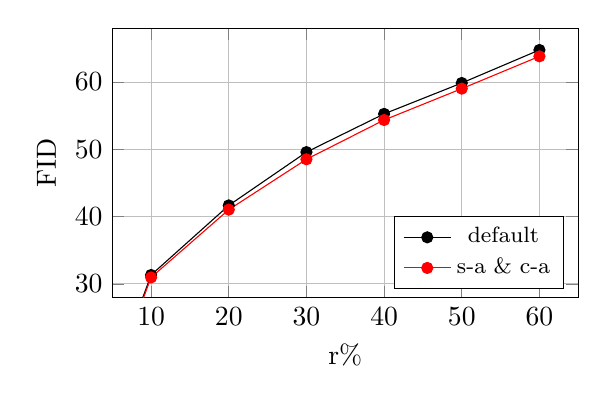
\begin{tikzpicture}
\begin{axis}[
    title={},
    height=5cm,
    width=7.5cm,
    xlabel={r\%},
    ylabel={FID},
    xmin=5, xmax=65,
    ymin=28, ymax=68,
    xtick={10,20,30,40,50,60},
    ytick={30,40,50,60},
    legend pos=south east,
    xmajorgrids=true,
    ymajorgrids=true,
    legend style={font=\footnotesize}
]

\addplot[
    color=black,
    mark=*
    ]
    coordinates {
    (0,0)(10,31.33)(20,41.67)(30,49.59)(40,55.27)(50,59.86)(60,64.77)
    };
    
\addplot[
    color=red,
    mark=*
    ]
    coordinates {
    (0,0)(10,30.97)(20,41.04)(30,48.52)(40,54.36)(50,59.02)(60,63.82)
    };
    
\legend{default, s-a \& c-a}
    
\end{axis}
\end{tikzpicture}